\chapter{Statistical results and interpretation}
\label{cha:statisticalResults}

In this section the statistical results and interpretations are discussed.
In Section~\ref{sec:likelihood} the likelihood model used to interpret the results of the \alphat search is
detailed and in Section~\ref{sec:results} the results of a maximum likelihood fit to the observed data presented. 
As no significant excess is seen the results are interpreted by setting uppoer limits at 95\% confidence 
level (CL) on the cross section of supersymmetric simplified models. The procedure for setting the limits and 
the results are detailed in Sections~\ref{sec:limits} and~\ref{sec:limits-sms} respectively.
In this section the \znunu background is labelled as \zInv~ while 
the \ttj~plus \wj~background is labelled as \ttW.

\section{Likelihood model}
\label{sec:likelihood}

The \alphat~analysis relies on control regions to predict the normalisation of category of \njet, \nb~and \scalht 
(which are in the following identified with \htcat) and on simulation to predict the shape 
of \mht~within each category. The likelihood model is split into hadronic and control components
linked by floating parameters for the prediction. In one \htcat~category, j, 
the hadronic component may be written as a multiple of Poisson likelihoods
for the observation in each \mht bin 
($\mathrm{Pois}(n|\lambda) \equiv e^{-n}\frac{\lambda^{n}}{n!}$):

\begin{multline}
\label{eq:hadronicLikelihood}
\mathcal{L}^{j}_{\mathrm{had}} = \prod_i \mathcal{L}^{j,i}_{\mathrm{had}} = \prod_i \mathrm{Pois}(n^{j,i}_{\mathrm{had}} |\, b^{j,i}_{\zInv~,had}\times\phi^{j}(\mu\rightarrow\zInv~)\times a^{j}\times\rho^{j,i}_{\zInv~,\mathrm{had}}\, + \\ 
b^{j,i}_{\ttW,\mathrm{had}}\times\phi^{j}(\mu\rightarrow\ttW)\times a^{j}\times\rho^{j,i}_{\ttW,\mathrm{had}}\, + b^{j,i}_{\text{QCD},\mathrm{had}}\times\omega^{j,i}_{\text{QCD},\mathrm{had}} + \,r\times s^{j,i}_{\mathrm{had}}\times\rho^{j,i}_{s,\mathrm{had}}) 
\end{multline}

where the product is over each \mht bin, i, for the \htcat~category, $b^{j,i}_{\zInv/\ttW,had}$ are the predicted number 
of events from simulation for the electroweak backgrounds; 
$b^{j,i}_{\text{QCD},had}$ are the predicted 
numbers for the QCD multijet component (from the method described in Section~\ref{sec:qcd-pred});
the $a^{j}$ parameter is unconstrained and connects the prediction of the signal region
to the control regions (see below); the $\phi^{j,i}$ contain the systematic uncertainties on the 
transfer factors from the data driven tests; the $\rho^{j}$ contain the systematics from 
variations in simulation, the systematics derived from the control regions on the~\mht shape 
and the uncertainty from the limited number of simulated events; 
$r$ is the unconstrained \emph{signal strength} parameter and $\omega_{\text{QCD},\mathrm{had}}$ 
contains the uncertainties on the QCD multijet component. 

The component of the likelihood for the \mj~control region, which is not categorised in \mht, can be written as

\begin{equation}
\label{eq:muLikelihood}
\mathcal{L}^{j}_{\mathrm{\mu}} = \mathrm{Pois}(n^{j}_{\mathrm{\mu}} |\, b^{j}_{\mu}\times a^{j}\times\rho^{j}_{\mu} +\, b^{j}_{\text{QCD},\,\mu} + \,r \times s^{j}_{\mathrm{\mu}}\times\rho^{j}_{s,\mu})
\end{equation}

similarly to Equation, $\rho^{j}_{\mu}$ contains the uncertainty in the \htcat from variations in simulation. The $s^{j}_{\mathrm{\mu}}$
encodes the signal \emph{contamination} in the control region which is small by design. The connection between the control and signal region
is encoded by the unconstrained $a^{j}$ parameter and the sub-dominant QCD component, $b^{j}_{\text{QCD},\,\mu}$, is taken from simulation. 

The \zInv~component in the signal region is also predicted using the \gj~and \mmj~regions. 
By rewriting $\phi^{j}(\mu\rightarrow\zInv~)\times a^{j}$ and $\phi^{j}(\mu\rightarrow\ttW)\times a^{j}$
as ${a'}(\mu\rightarrow\zInv~)$ and $a'(\mu\rightarrow\ttW~)$ respectively, the connections to the \gj~and \mmj~regions
may be written as, 

\begin{align}
\label{eq:mumuGammaLikelihood}
\mathcal{L}^{j}_{\mathrm{\mu\mu}} &= \mathrm{Pois}(n^{j}_{\mathrm{\mu\mu}} |\, b^{j}_{\mu\mu}\times 
\left({a'}^{j}/\phi^{j}(\mu\mu\rightarrow\zInv~)\right)\times\rho^{j}_{\mu\mu} +\,b^{j}_{\text{QCD},\,\mu\mu} + \,r\times s^{j}_{\mathrm{\mu\mu}}\times\rho^{j}_{s,\mu\mu}) \\
\mathcal{L}^{j}_{\mathrm{\gamma}} &= \mathrm{Pois}(n^{j}_{\mathrm{\gamma}} |\, b^{j}_{\gamma}\times 
\left({a'}^{j}/\phi^{j}(\gamma\rightarrow\zInv~)\right)\times\rho^{j}_{\gamma} + \,b^{j}_{\text{QCD},\,\gamma} + \,r\times s^{j}_{\mathrm{\gamma}}\times\rho^{j}_{s,\gamma})
\end{align}

where parameters are defined as in Equations~\ref{eq:hadronicLikelihood} and~\ref{eq:muLikelihood}. 
In these equations the $\phi^{j}$ appear on the denominator as the connection between the control and signal region is 
inverted.

The modifier and constraint terms of the parameters representing the systematic uncertainties and 
connections between control and signal regions, \emph{nuisance parameters}, can be summarised as,
\begin{itemize}
\item The transfer factor systematics and uncertainties on the QCD multijet contribution 
are taken to be \emph{log normal} uncertainties such that the logarithm of the variable has 
a Gaussian (normal) constraint~\cite{templateMorphing}. These uncertainties are correlated per topology and \scalht bin 
(pair of \scalht bin for uncertainties derived using \mmj)
\item The systematic uncertainties from variations in simulation and those derived on the \mht~shape from the control regions 
are included using \emph{vertical template morphing}~\cite{templateMorphing}. For vertical template morphing, the yield
in each bin is interpolated quadratically between the $\pm 1\sigma$ variations for each source of
uncertainty and extrapolated linearly beyond this range. The constraint term is Gaussian
with mean 0 and width 1. The uncertainties from simulation and those derived from the control regions
are fully correlated and uncorrelated across all categories respectively.
\item The Poisson uncertainty due to the limited number of simulated events is approximated using
two parameters per bin which multiply the total background and signal contributions and which 
are Gaussian constrained. These uncertainties are fully uncorrelated across all categories.
\end{itemize}

The total likelihood can be written as a product over all \htcat~bins,

\begin{equation}
\label{eq:totalLikelihood}
\mathcal{L} = \prod_{j\in\htcat} \mathcal{L}^{j}_{\mathrm{had}} \times \mathcal{L}^{j}_{\mathrm{\mu\mu}} 
\times \mathcal{L}^{j}_{\mathrm{\gamma}} \times \mathcal{L}^{j}_{\mathrm{\mu}}
\end{equation}


\section{Results of the fit to data}
\label{sec:results}
The expected number of events from the Standard Model backgrounds are determined from 
a simultaneous fit over all parameters using data from the control regions only, \emph{CR-only fit},
as well as using data from all regions, \emph{full fit}. The CR-only fit provides the 
best representation of the background predictions of the \alphat~search from the control regions.

In Figures~\ref{fig:mono},~\ref{fig:asym} and~\ref{fig:sym} the results of the CR-only fit and the full fit are presented in all \scalht, \njet 
and \nb~categories under a standard model only hypothesis (r = 0) for the monojet, asymmetric 
and symmetric categories respectively. No significant tension is observed between the predictions
and data. Additionally, in Figure~\ref{fig:mht-templates}, the distribution in \mht for representative 
categories of \scalht, \njet and \nb, sensitive to hadronic SUSY models with \TeV ~scale squarks and gluinos, 
shows good agreement between prediction and data.

The fine binned categorisation can complicate the comprehension of the global agreement between data and 
prediction across the signal region. In Section~\ref{sec:agg-reg} the result is presented using 
\emph{aggregated regions} in which the categorisation is merged. 

\begin{figure}[!h]
  \begin{center}
    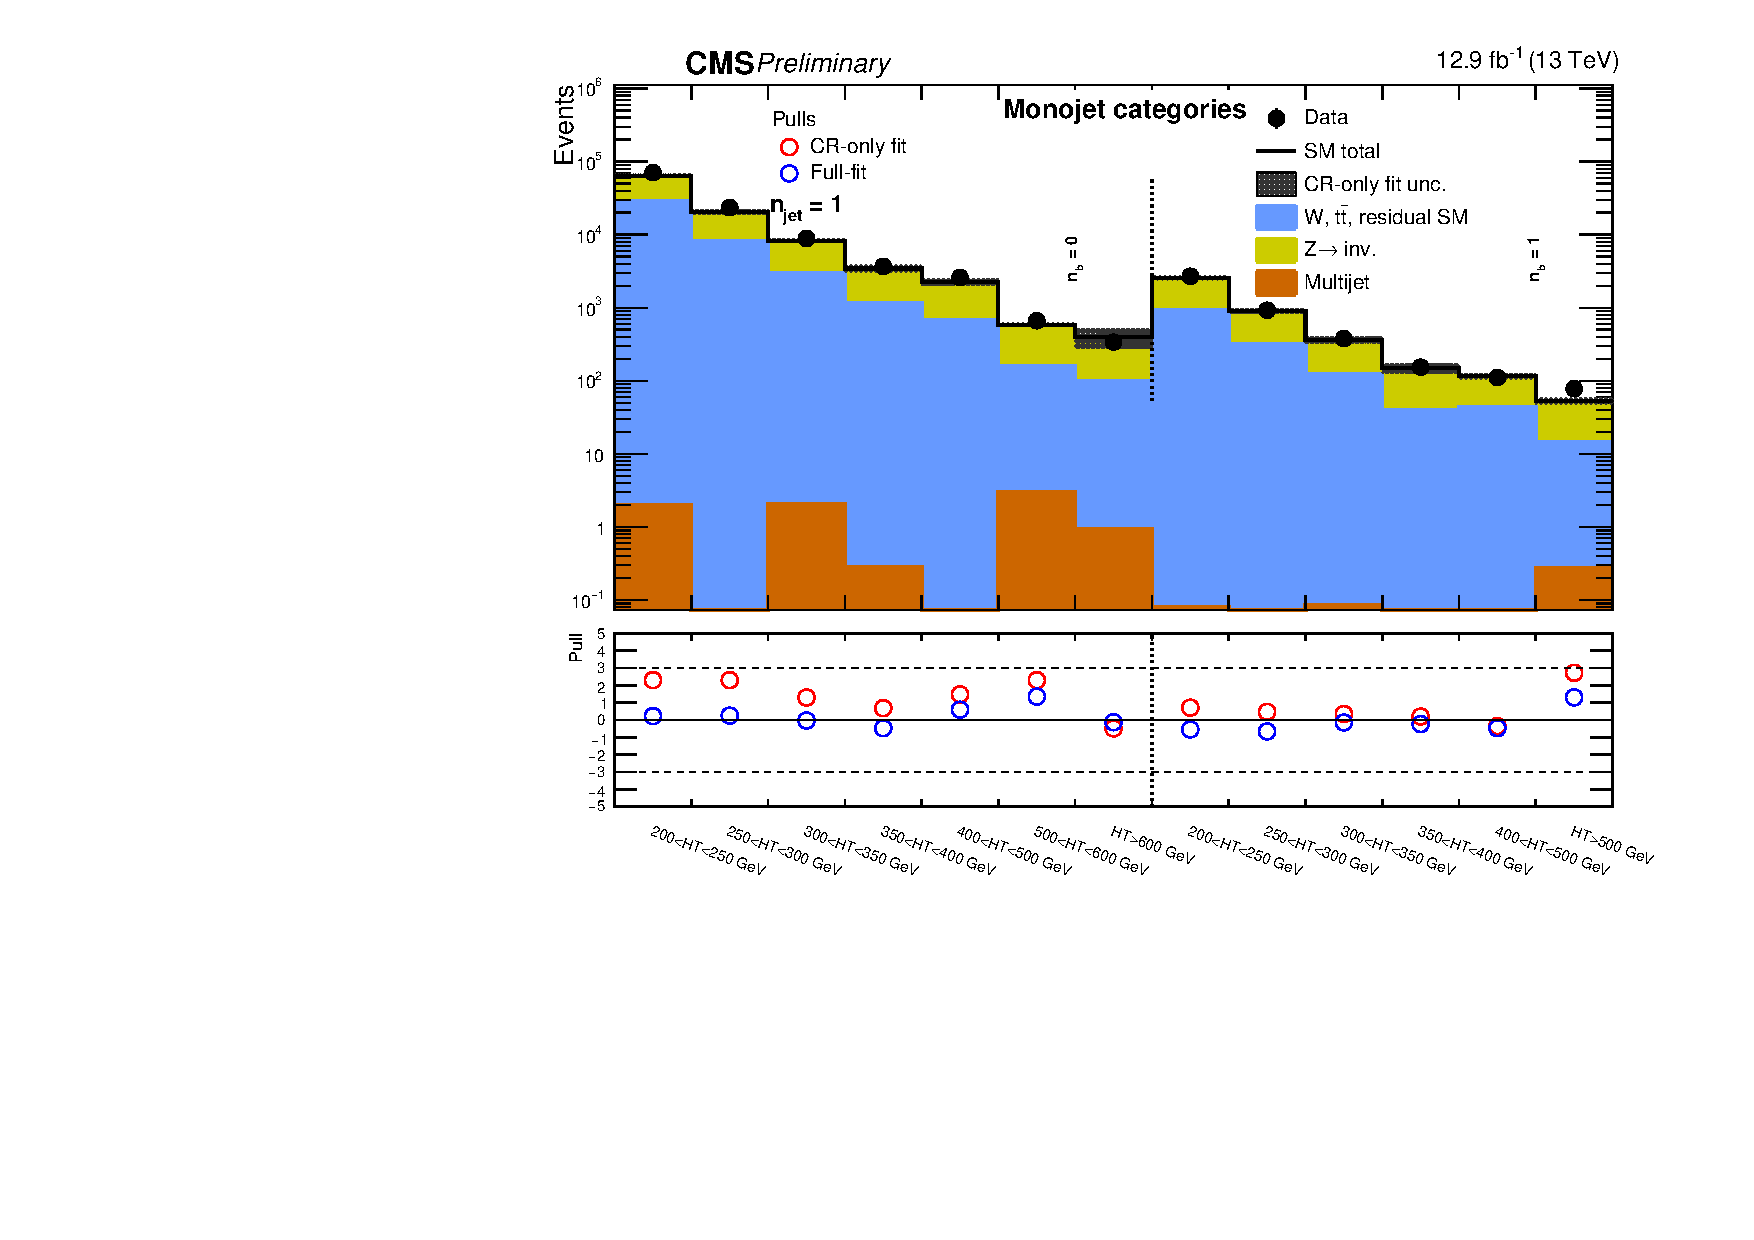
\includegraphics[width=0.7\textwidth]{Figures/statisticalResults/summaryPlot_Monojet_prefit_overlay_fit_b}
    \caption{Top panel: event yields observed in data (solid circles) 
	with their associated Poisson uncertainties represented by error bars 
	are compared to SM predictions with associated uncertainties (black
      histogram with shaded band) from a CR-only fit as a function of
      \nb and \scalht for the monojet topology in the
      signal region. Bottom panel: the significance of deviations
      (pulls) observed in data with respect to the SM expectations
      from the CR-only (red circles) and full fit (blue circles). The
      pulls are indicative only and cannot be considered
      independently.}
    \label{fig:mono}
  \end{center}
\end{figure}

\begin{figure}[!h]
  \begin{center}
    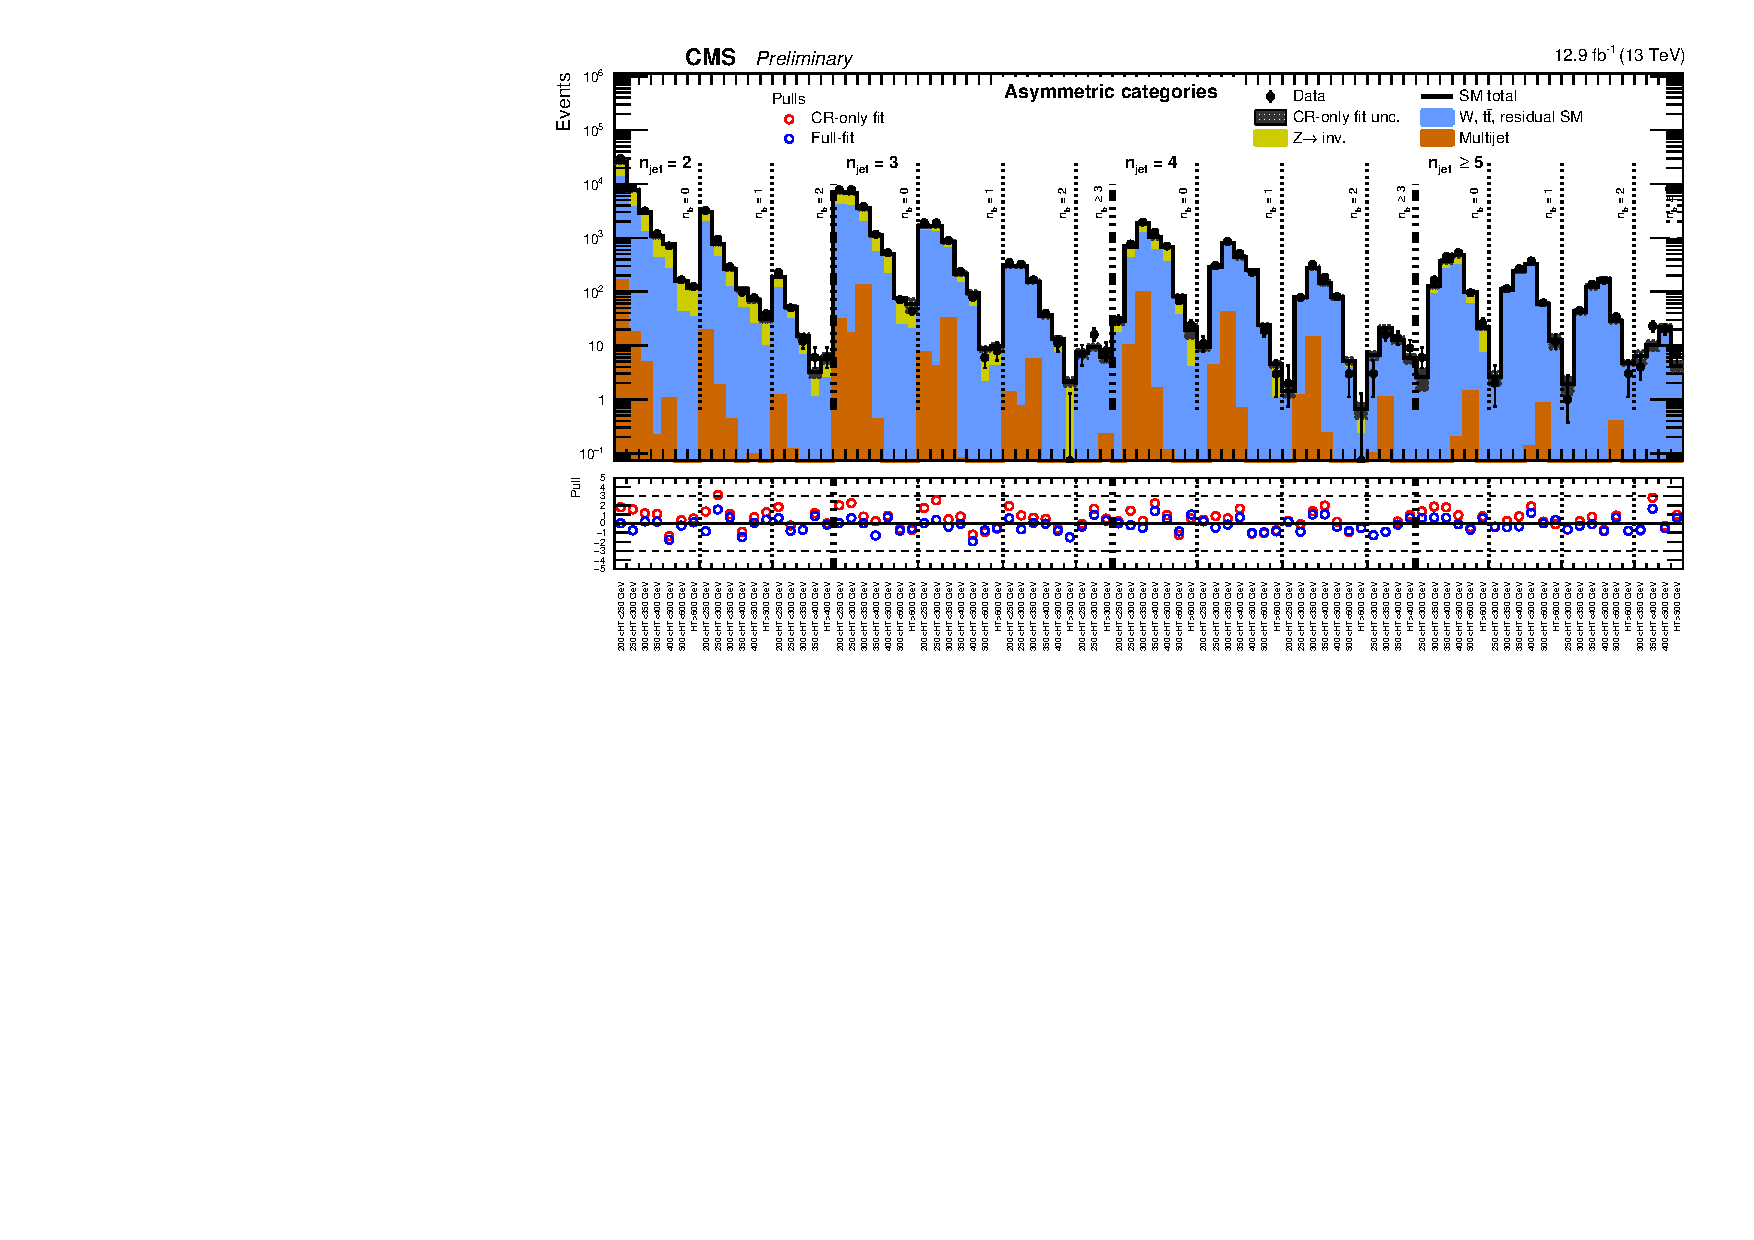
\includegraphics[angle=90,width=0.7\textwidth]{Figures/statisticalResults/summaryPlot_Asymmetric_prefit_overlay_fit_b}
    \caption{Top panel: event yields observed in data (solid circles) 
	with their associated Poisson uncertainties represented by error bars 
	are compared to SM predictions with associated uncertainties (black
      histogram with shaded band) from a CR-only fit as a function of
      \njet, \nb and \scalht for the asymmetric topology in the
      signal region. Bottom panel: the significance of deviations
      (pulls) observed in data with respect to the SM expectations
      from the CR-only (red circles) and full fit (blue circles). The
      pulls are indicative only and cannot be considered
      independently.}
    \label{fig:asym}
  \end{center}
\end{figure}

\begin{figure}[!h]
  \begin{center}
    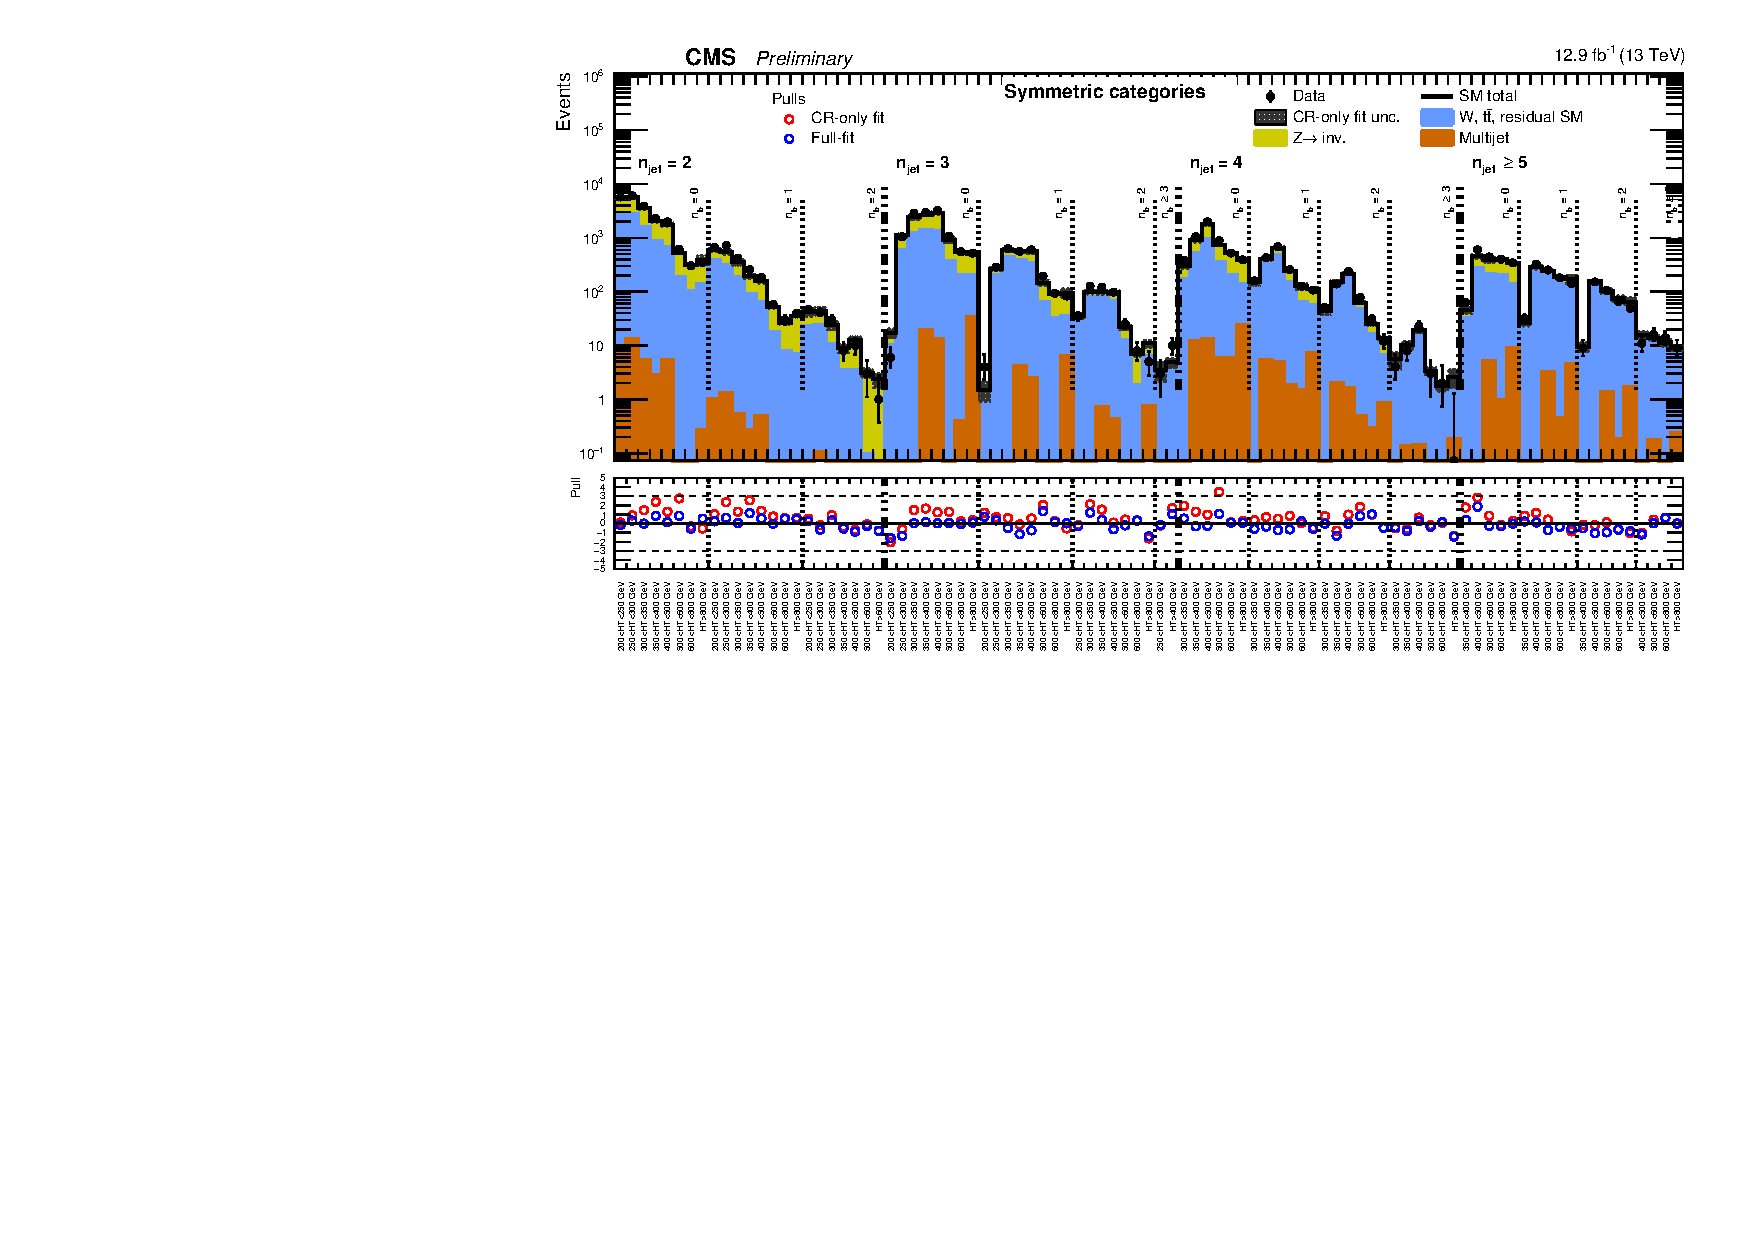
\includegraphics[angle=90,width=0.7\textwidth]{Figures/statisticalResults/summaryPlot_Symmetric_prefit_overlay_fit_b}
    \caption{Top panel: event yields observed in data (solid circles) 
	with their associated Poisson uncertainties represented by error bars 
	are compared to SM predictions with associated uncertainties (black
      histogram with shaded band) from a CR-only fit as a function of
      \njet, \nb and \scalht for the symmetric topology in the
      signal region. Bottom panel: the significance of deviations
      (pulls) observed in data with respect to the SM expectations
      from the CR-only (red circles) and full fit (blue circles). The
      pulls are indicative only and cannot be considered
      independently.}
    \label{fig:sym}
  \end{center}
\end{figure}

\begin{figure}[!tbhp]
  \begin{center}
    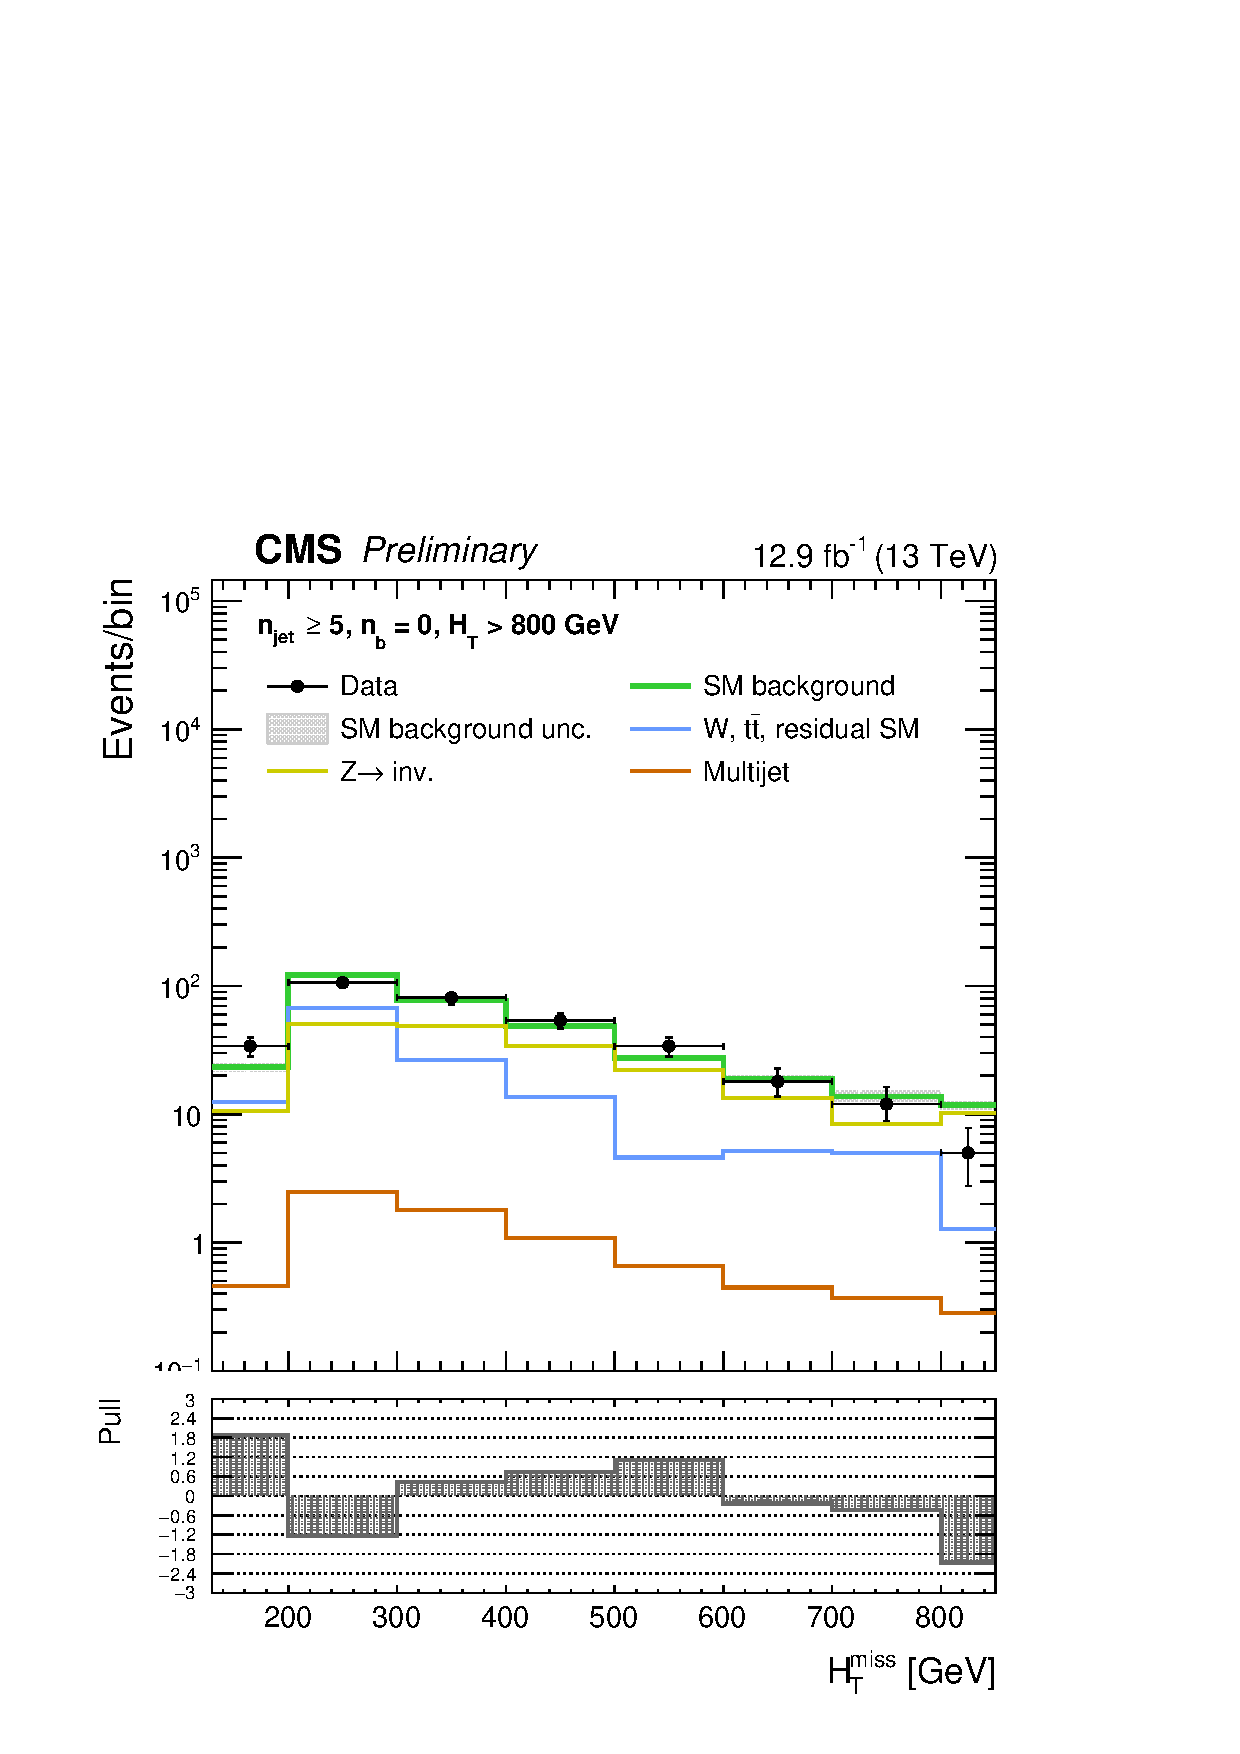
\includegraphics[width=0.45\textwidth]{Figures/statisticalResults/mhtShape_eq0b_ge5j_800_Inf_fit_b.pdf} 
    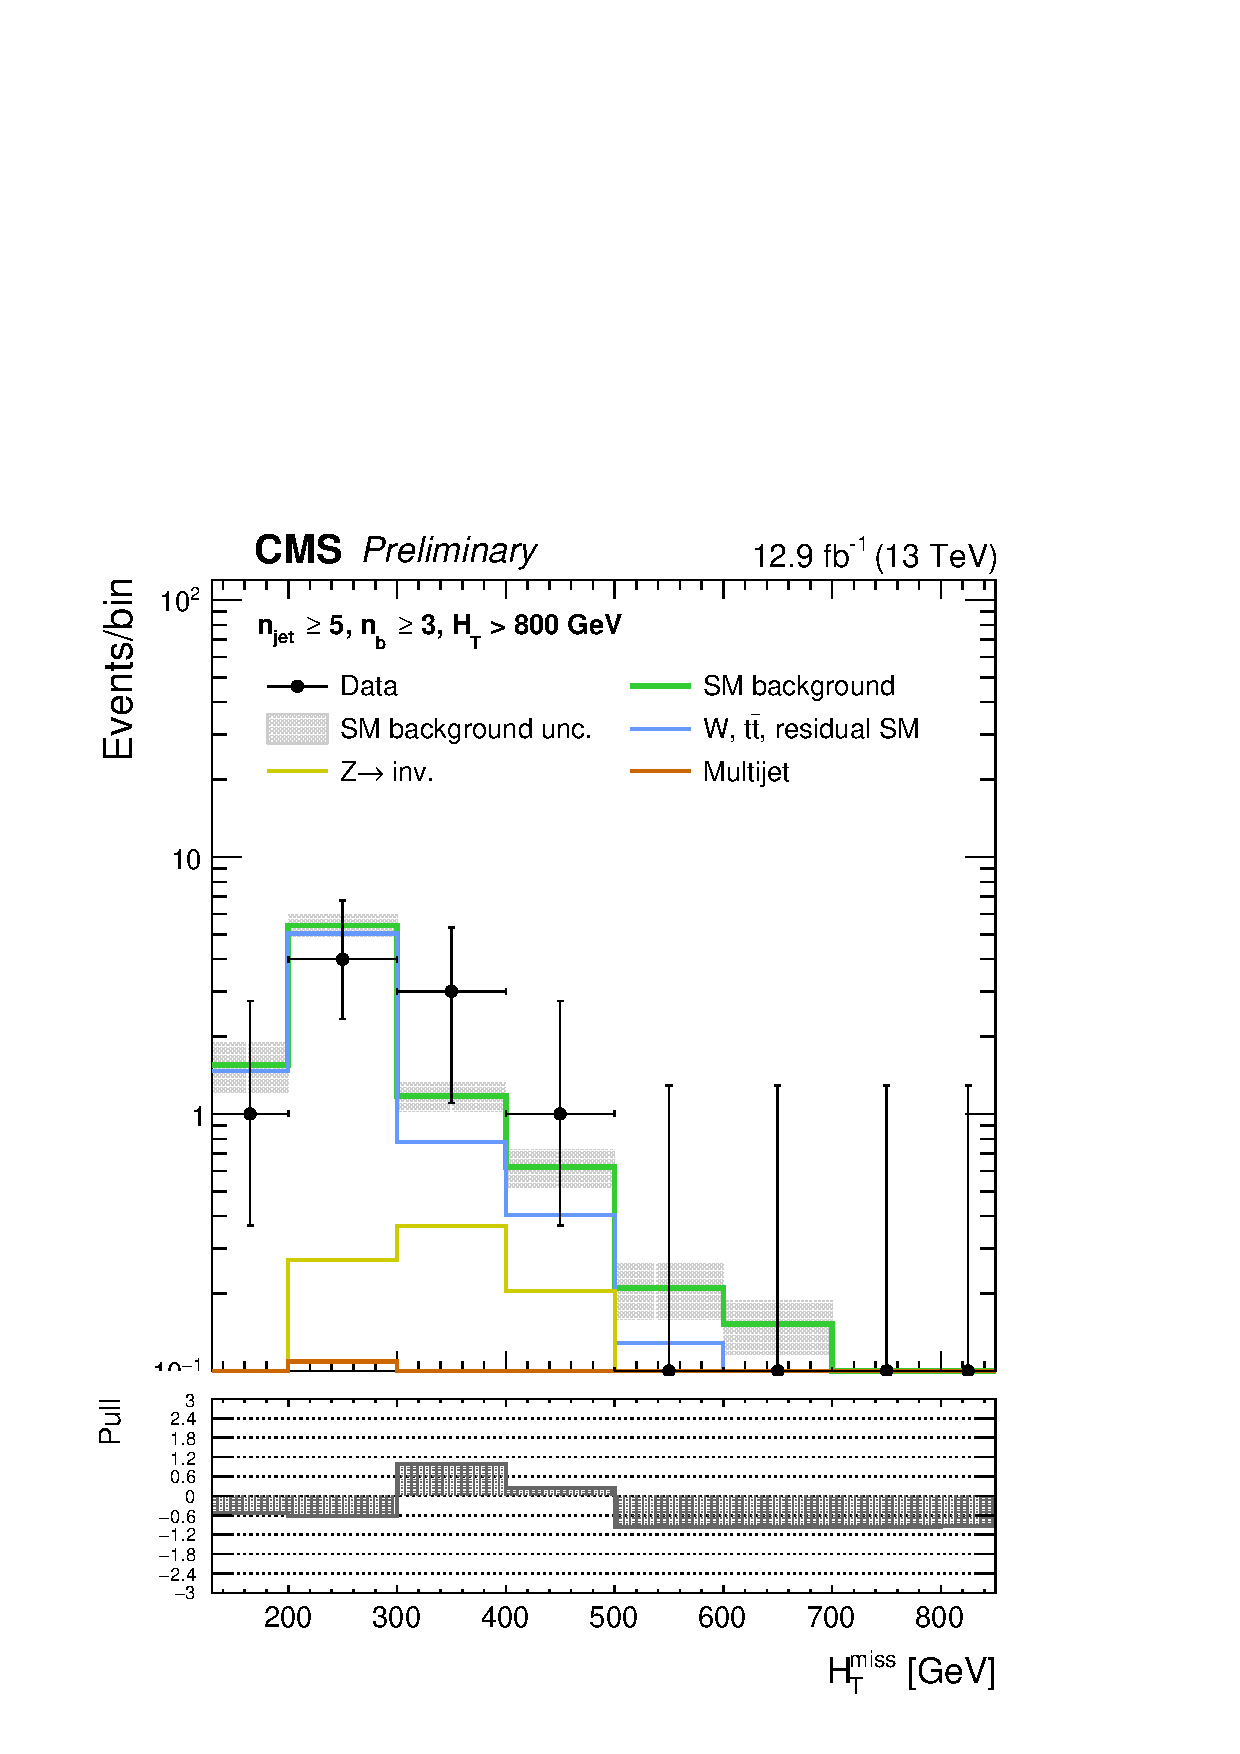
\includegraphics[width=0.45\textwidth]{Figures/statisticalResults/mhtShape_ge3b_ge5j_800_Inf_fit_b.pdf} 
  \end{center}
  \caption{Event yields observed in data (solid circles) and SM
    expectations from the CR-only fit with their associated
    uncertainties (green histogram with shaded band) as a function of
    \mht for events in the signal region that satisfy $\njet \geq
    5$, $\scalht > 800\GeV$, and (Left) $\nb = 0$ or (Right) $\nb \geq
    3$. The final bin is the overflow bin. The bottom panels indicate
    the significance of the deviations (pulls) observed in data with respect
    to the SM expectations, expressed in terms of the total
    uncertainty in the SM expectations. The pulls are indicative only
    and cannot be considered independently.  
    \label{fig:mht-templates} 
  }
\end{figure}

\clearpage
\section{Interpretation}

Given the agreement between prediction and results presented in Section~\ref{sec:results}, no evidence
for physics beyond the standard model is observed. The results are therefore used to constrain
the parameter space of simplified supersymmetric models. The simplified 
models considered are the gluino-mediated and direct production of
both bottom and top squark pairs. The \alphat~search is expected to be particularly
sensitive to such topologies due to the significant hadronic activity, bottom quarks, jet multiplicity
and \mht that may be present in the final state. Limits at 95\% confidence level (see Section~\ref{sec:limits}) 
are set on the production cross section of each model.

\subsection{Procedure for deriving limits}
\label{sec:limits}

This section outlines the procedure for deriving the upper limits on the signal 
strength at 95\% confidence level. A more comprehensive treatment can be found in~\cite{asymp}.

In the following section the signal strength is considered to be the parameter of interest
and all other parameters in the fit are termed the \emph{nuisance parameters} ($\boldsymbol{\theta}$). Considering
the likelihood defined in Equation~\ref{eq:totalLikelihood}, the profile likelihood ratio can be defined as

\begin{equation}
\label{eq:profile}
q(r) = \frac{\mathcal{L}(r,\hat{\boldsymbol{\theta}}(r))}{\mathcal{L}(\hat{r},\hat{\boldsymbol{\theta}})},
\end{equation}

where $\hat{\boldsymbol{\theta}}$ and $\hat{r}$ are the values of $\boldsymbol{\theta}$ and $r$ that maximise $\mathcal{L}$
, maximum-likelihood (ML) estimators, while $\hat{\boldsymbol{\theta}}(r)$ is the value
of $\boldsymbol{\theta}$ that maximises $\mathcal{L}$ for the specified value of $r$. 

Given that $r < 0$ is unphysical the profile likelihood is modified to
\begin{equation}
\label{eq:profileNew}
\tilde{q}(r) = 
\begin{cases}
q(0)\quad r \le 0, \\ 
q(r)\quad r > 0. \\ 
\end{cases}
\end{equation}

The test statistic used to derive the upper limit on $r$ can then be defined as

\begin{equation}
t_r = 
\begin{cases}
-2\,\text{ln}\,\tilde{q(r)}\quad &\hat{r} \le r, \\ 
0 \quad &\hat{r} > r. \\ 
\end{cases}
\end{equation}

Considering Equation~\ref{eq:profile}, $t_r$ will be zero at the ML value of $r$.
Increasing values of $t_r$ represent lesser compatibility of that value of $r$ with
the observed data. The test statistic is set to zero for $\hat{r} > r$ as
values of $r$ less than $\hat{r}$ are not part of the \emph{rejection region} for upper limits. 

The probability density function, $f(t_r|r)$, for $t_r$ may be built by 
generating pseudo-experiments or approximated using the asymptotic formulae 
detailed in~\cite{asymp}. The \alphat~analysis uses the asymptotic
approximation for $f(t_r|r)$. The \textit{p}-value, $p_r$, is defined as

\begin{equation}
p_r = \int_{t_{r,obs}}^{\infty}\, f(t_r|r)\, dt_r
\end{equation}

where ${t_{r,obs}}$ is the observed value of the test statistic. Finally,
the $\text{CLs}$ is defined as

\begin{equation}
\text{CLs}(r) = \frac{p_r}{1-p_0}.
\end{equation}

The upper limit on $r$ is defined as the value of $r$ which corresponds to 
$\text{CLs}(r) = 0.05$ ($r_{95}$). Values of $r$ greater than this are said to be excluded at 95\%
confidence level.

The expected limit on a given signal strength, $r_{95}^{exp}$, is defined by the median value of the distribution
of $r_{95}$ built from pseudo datasets generated with no signal contribution (r = 0). The variation in the 
expected limit may also be estimated by the relevant quantiles from this distribution.
For the \alphat~analysis, the value and variations of $r_{95}^{exp}$ are approximated using 
the asymptotic formulae detailed in~\cite{asymp}.

\subsection{Signal model contribution and systematic uncertainties}

The experimental efficiency times acceptance ($\epsilon \times A$) in both the signal and 
control regions is derived independently for each signal model for each gluino or squark 
mass ($m_{\text{SUSY}}$) and neutralino mass ($m_{\tilde{\chi}^{0}}$). As for the 
background processes, the simulated events for the signal contribution are corrected for 
jet energy corrections, b tag scale factors, lepton scale factors, pile up modelling and trigger efficiencies.
In addition, a correction is made to account for differences observed in the initial 
state radiation modelling between data and simulation. Systematic uncertainties are included 
on each of these corrections, analogously to the background processes. The signal contribution
cannot be predicted using data and therefore the overall normalisation contains an uncertainty
from the luminosity measurement of 6.2\%. All systematics are summarised
in Table~\ref{tab:signal_systs} including typical magnitudes for direct bottom squark production.

\begin{table}[h!]
  \caption{
    Representative magnitudes of systematic uncertainties in the
    experimental acceptance for simplified models that assume the 
    pair production of bottom squarks and their decay to a b
    quark and a \chiz.}  
  \label{tab:signal_systs}
  \centering
  \footnotesize
  \begin{tabular}{ lccc }
    \hline
    Systematic source\T\B          & Correlated & Typical magnitude (\%) \\
    \hline
    Luminosity\T                   & Yes        & 6.2                    \\
    Monte Carlo statistics         & No         & 1--50                  \\
    Jet energy scale               & Yes        & 3--10                  \\
    b tag efficiency scale factors & Yes        & 5--40                  \\
    Lepton scale factors           & Yes        & 1--5                   \\
    Pile-up                        & Yes        & 0--5                   \\
    Trigger efficiency             & Yes        & 0--4                   \\
    Initial state radiation        & Yes        & 1--20                  \\
%    Renormalisation/factorisation & Norm. + shape & No         & 10                     \\
    \hline
  \end{tabular}
\end{table}


\subsection{Upper limits on signal production cross section}
\label{sec:limits-sms}
In Figure~\ref{fig:limits-sms} the upper limits at 95\% CL set on the production cross section are shown
in the ($m_{\text{SUSY}}$, $m_{\tilde{\chi}^{0}}$) plane for the models considered.
Also shown are the expected and observed contours of $r_{95} = 1$ (models \emph{excluded}
at 95\% CL), the $\pm$ 1 and 2 $\sigma$ variations in the expected limit, and the observed limit under $\pm$ 1 $\sigma$ 
variations in the theoretical cross section uncertainty.

\begin{figure}[thp!]
  \begin{center}
    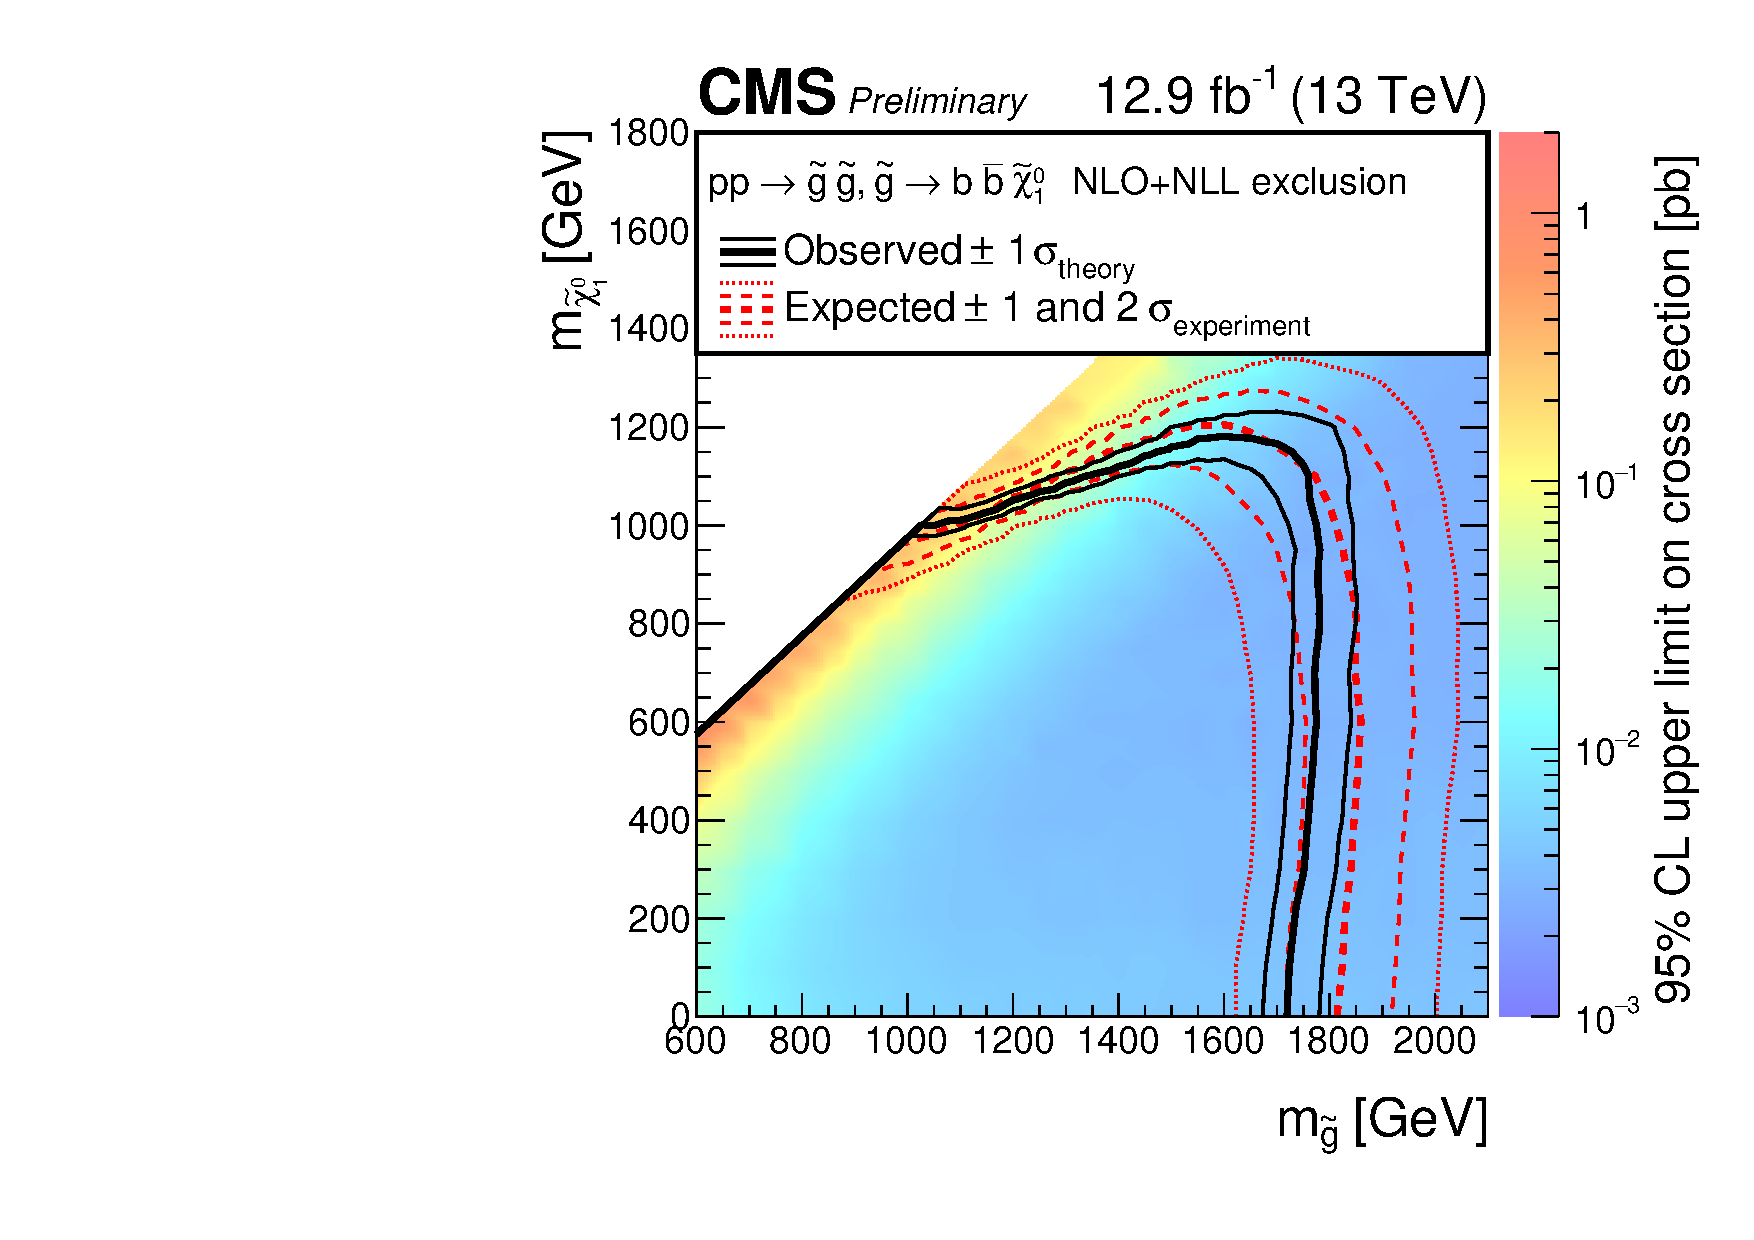
\includegraphics[width=0.45\textwidth]{./Figures/statisticalResults/SUS16T1bbbbXSEC.pdf} ~
    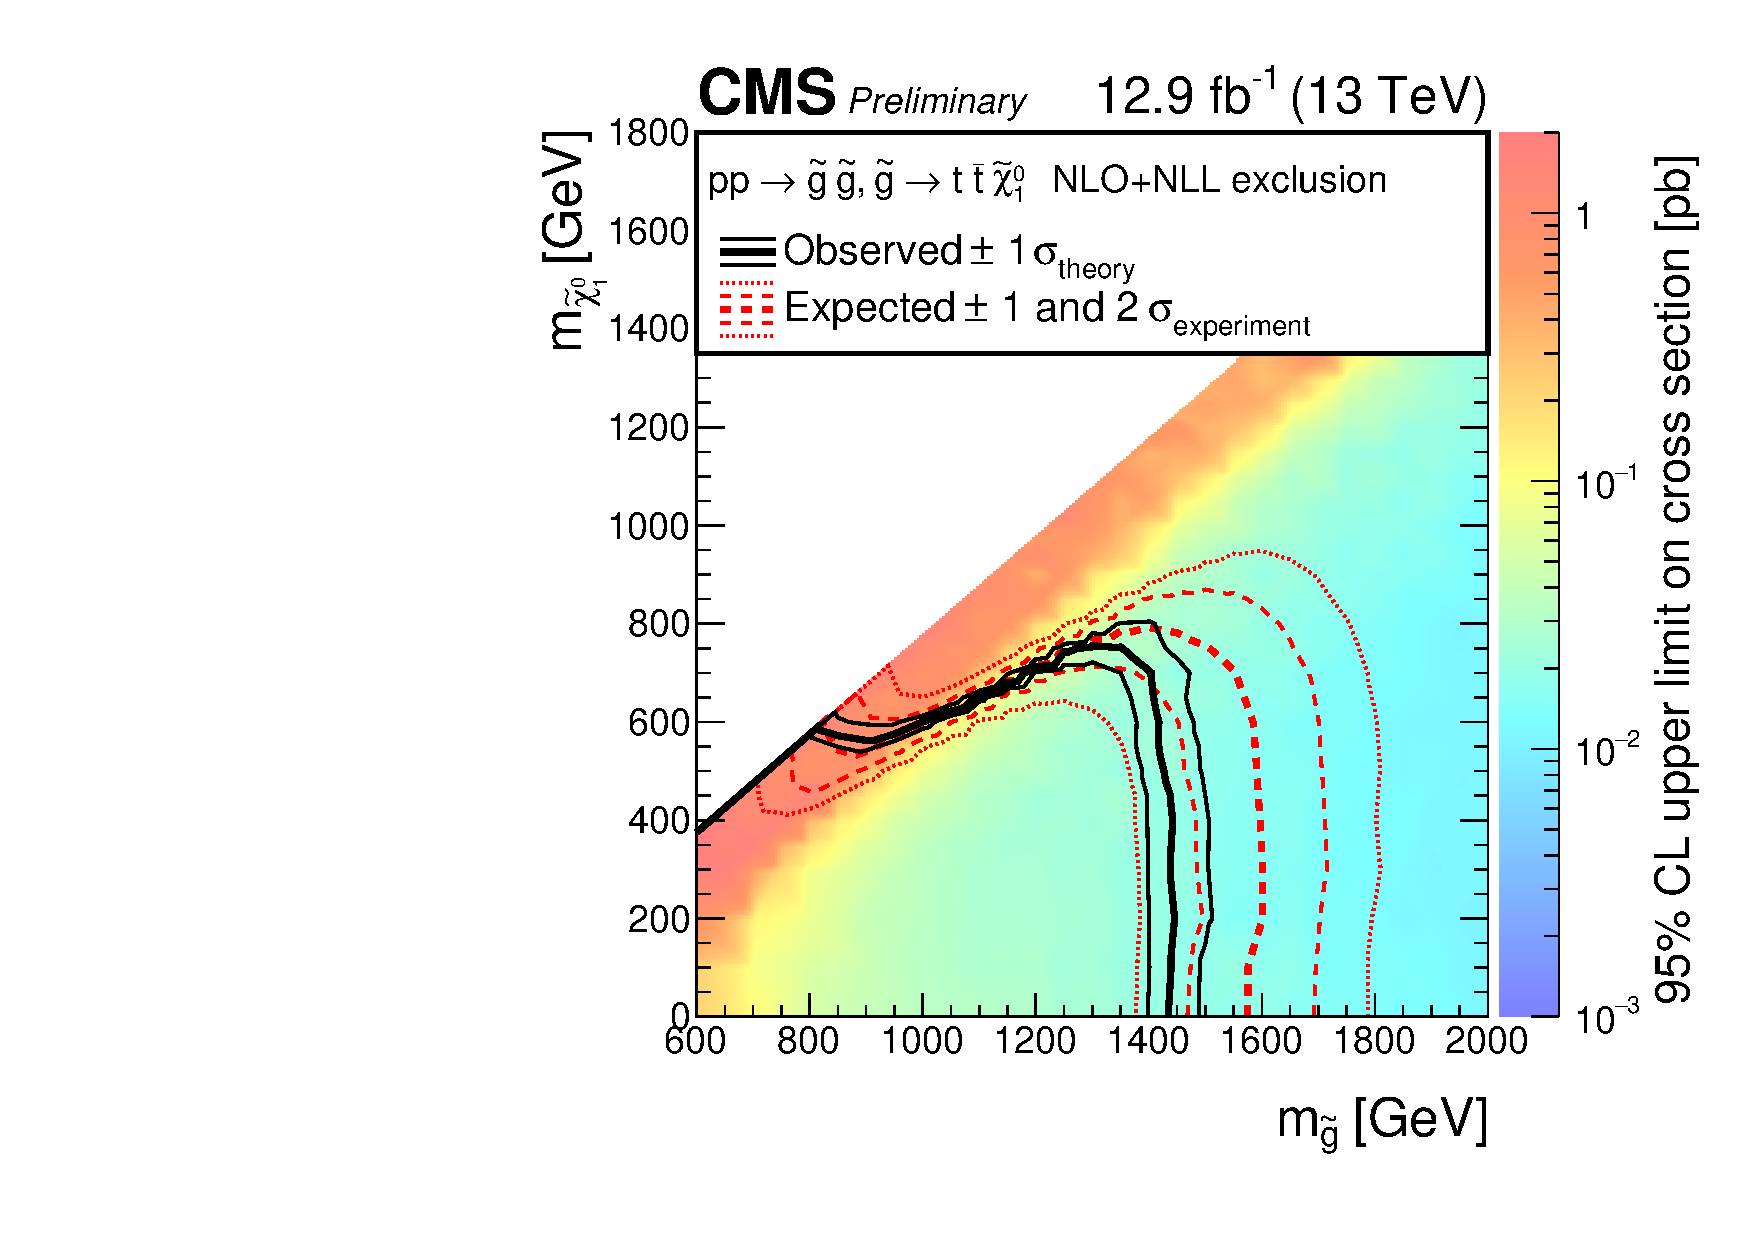
\includegraphics[width=0.45\textwidth]{./Figures/statisticalResults/SUS16T1ttttXSEC.pdf} \\
    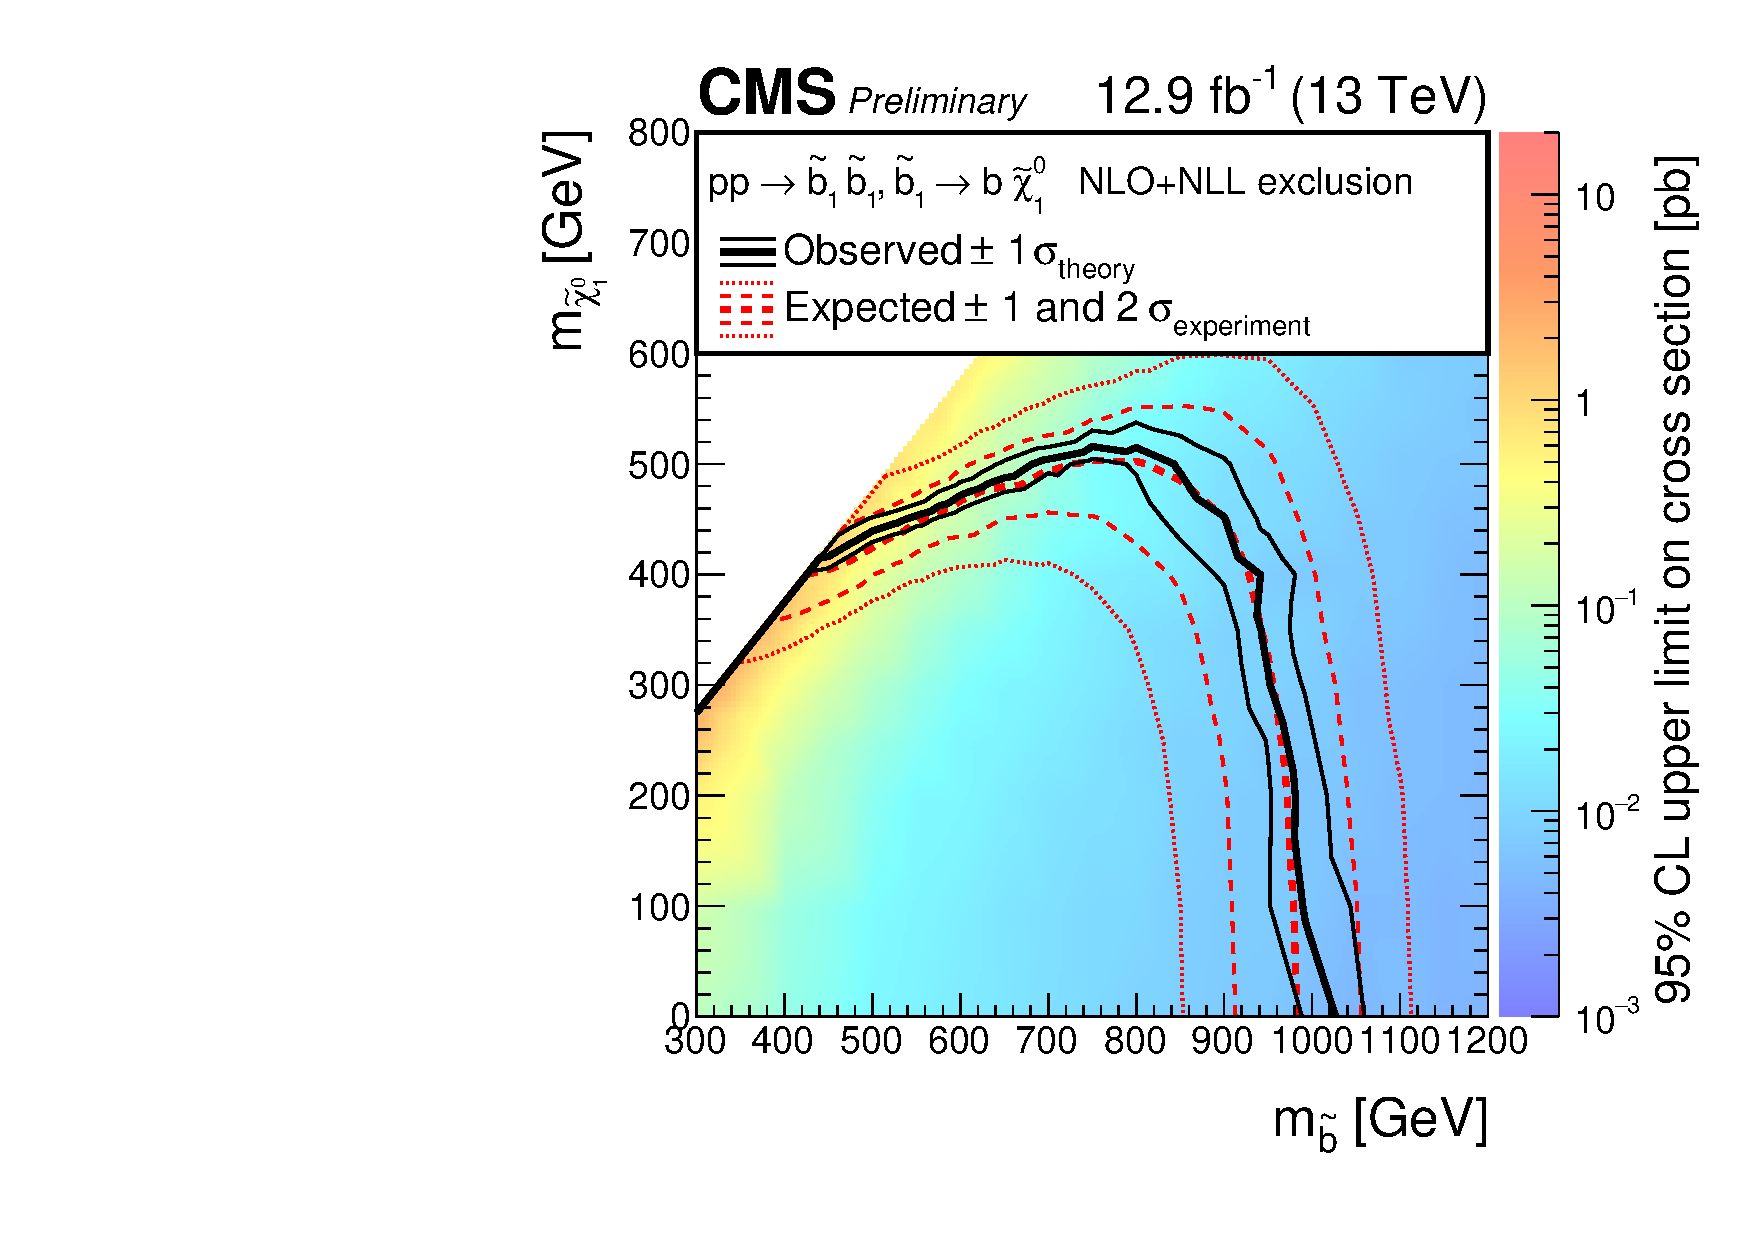
\includegraphics[width=0.45\textwidth]{./Figures/statisticalResults/SUS16T2bbXSEC.pdf} ~
    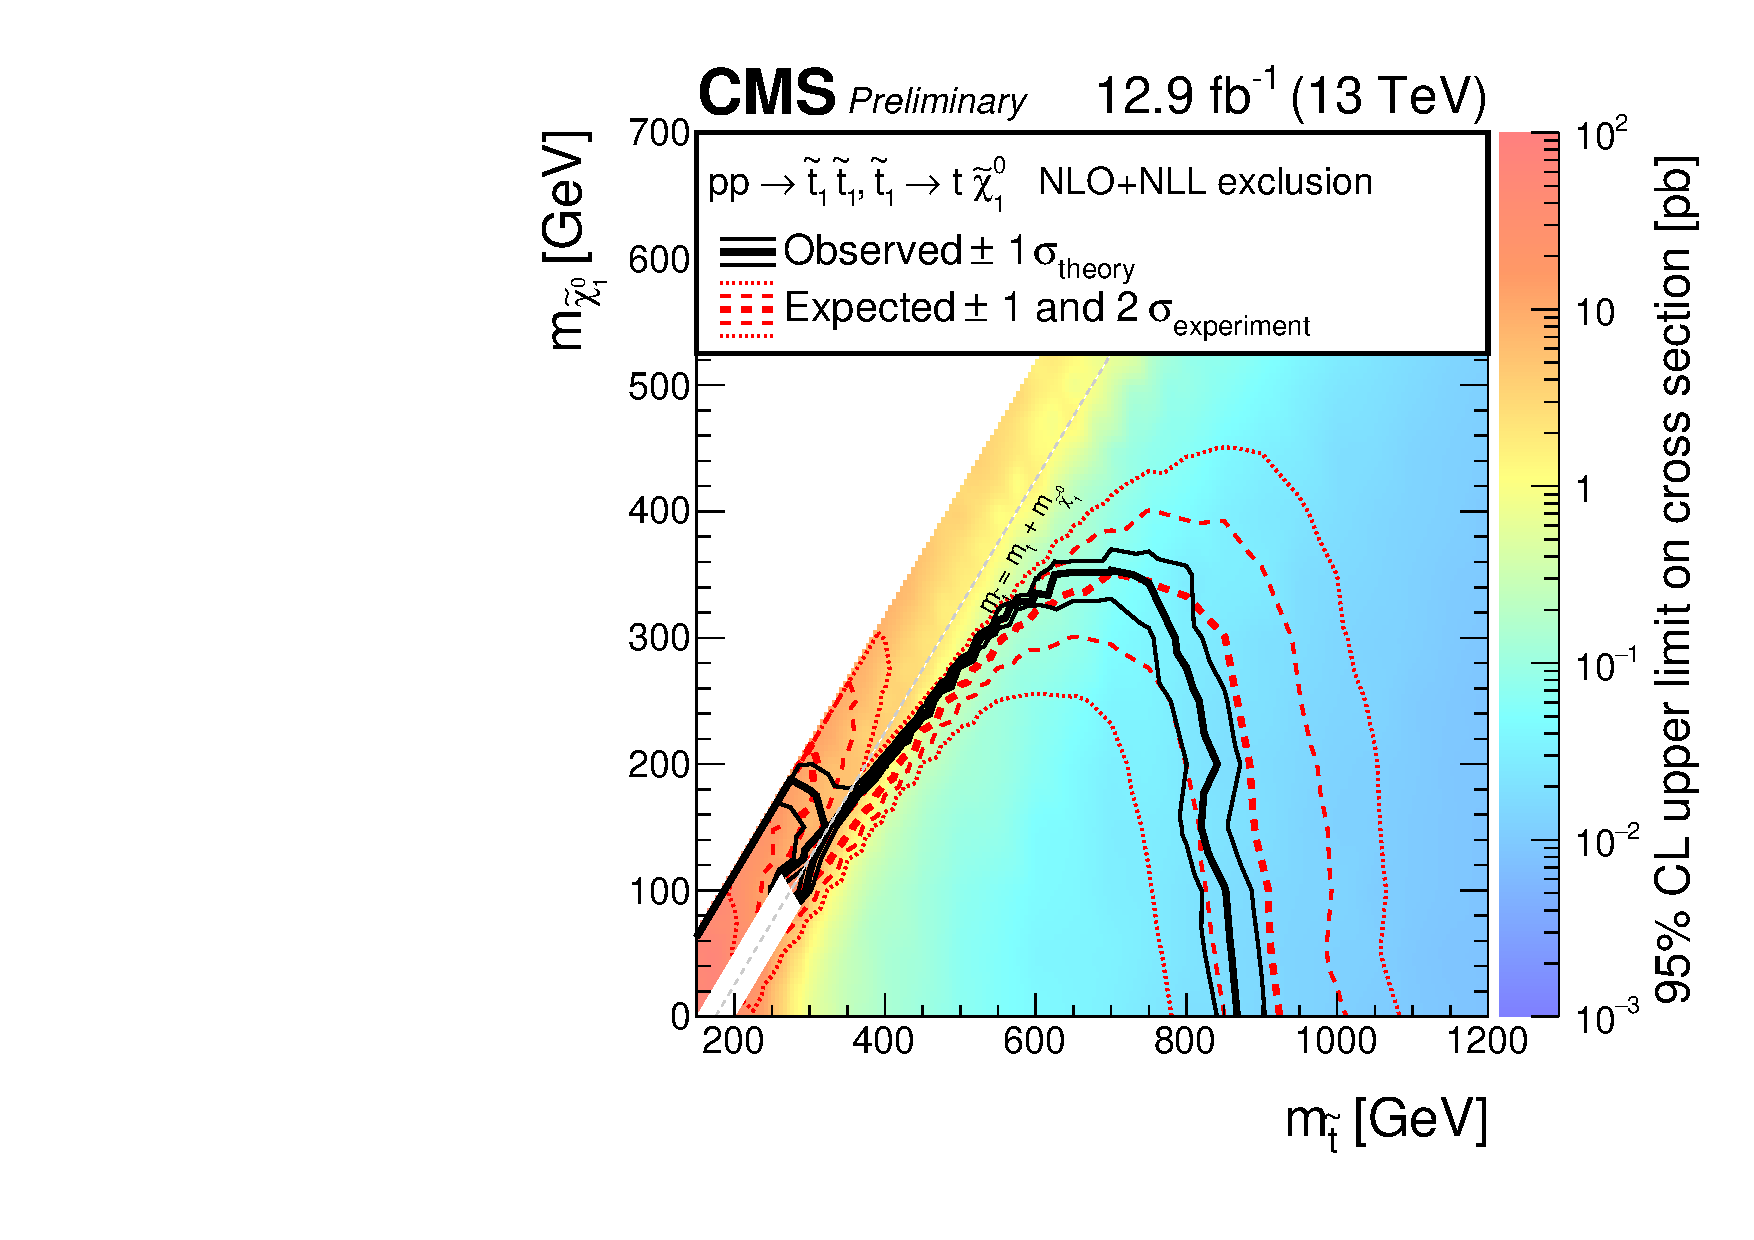
\includegraphics[width=0.45\textwidth]{./Figures/statisticalResults/SUS16T2ttXSEC.pdf} 
    \caption{Observed upper limit in cross section at 95\% confidence
      level (indicated by the colour scale) for simplified models that
      assume the (Top) gluino-mediated or (Bottom) direct production
      of (Left) bottom or (Right) top squark pairs, as a function of
      the gluino or squark mass and the $\chiz_{1}$ 
      mass. The black solid thick (thin) line indicates the observed
      mass exclusion regions assuming the nominal (${\pm}1 \sigma$
      theory uncertainty) production cross section. The red dashed
      thick (thin) line indicates the median (${\pm}1 \sigma$
      experimental uncertainty) expected mass exclusion
      regions. 
      \label{fig:limits-sms} }
  \end{center}
\end{figure}

\section{Summary}

The results of the~\alphat analysis with 12.9 \ifb of pp collision data have shown no significant
evidence of BSM physics. Upper limits at 95\% CL have therefore been set on a range 
of supersymmetric simplified models. In Table~\ref{tab:simplified-models-limits}, the highest mass 
of squark or gluino and \chiz~excluded at 95\% confidence level are shown for each model and compared to the highest
values excluded by searches on the full 7 and 8 \TeV~Run 1 CMS datasets. 
A significant increase in reach is achieved of 100 - 400 \GeV~in the
squark/gluino mass and 50 - 425 \GeV~in the mass of the \chiz. 

The improvements in sensitivity are driven by both the increase in the 
centre of mass energy and by improvements in the analysis strategy. Such improvements
include the addition of the \mht~dimension and the use of the \mj~control region
to predict~\zInv.

In Figure~\ref{fig:limits-sms-competition},
the reach of the \alphat search for the gluino-mediated and direct bottom
squark production is compared to two other hadronic searches for new physics on the 
same 12.9 \ifb dataset. The~\alphat search has comparable reach across the mass
plane and is particularly sensitive for high \chiz~masses.

The results presented in this section may be used to derive limits on BSM physics models 
not considered for this thesis. Such \emph{re-interpretations} of the \alphat search 
are discussed in Chapter~\ref{cha:simplifiedLikelihood}.

\newcommand{\ph}{\ensuremath{\phantom{1}}}
\begin{table}[tb]
  \caption{Summary of the mass limits obtained for the four 
    classes of simplified models. The limits indicate the strongest
    observed (expected) mass exclusions for the gluino or squarks, and
    $\chiz_1$, and the quoted values have uncertainties of
    $\pm$25\GeV.  
  }
  \label{tab:simplified-models-limits}
  \centering
  \footnotesize
  \begin{tabular}{ llcccc }
    \hline
		    &     	    & \multicolumn{4}{c}{Strongest obs. (exp.) mass exclusion [\GeV]}\T\B \\
    Production mode & Squark        &  \multicolumn{2}{c}{\alphat (13 \TeV)} \T\B & \multicolumn{2}{c}{Run 1 (7 \TeV ~+ 8 \TeV)}\T\B \\
    \cline{3-4}\cline{5-6}                                                                                        
                    &               & Gluino or squark\T\B & \chiz                                       & Gluino or squark\T\B & \chiz                                               \\
    \hline                                                                                               
    Gluino-mediated & Bottom        & 1775 \ph(1850)       & 1175 \ph(1200)                              & 1375  & \ph725                               \\ 
    Gluino-mediated & Top           & 1450 \ph(1600)       & \ph750 \ph\ph(800)                          & 1325  & \ph625                              \\ 
    Direct          & Bottom        & 1025 \ph\ph(975)     & \ph525 \ph\ph(500)                          & \ph725  &\ph325                               \\ 
    Direct\B        & Top           & \ph875 \ph\ph(925)   & \ph350 \ph\ph(350)                          & \ph775  & \ph300                              \\
    \hline
 \end{tabular}
\end{table}

\begin{figure}[thp!]
  \begin{center}
    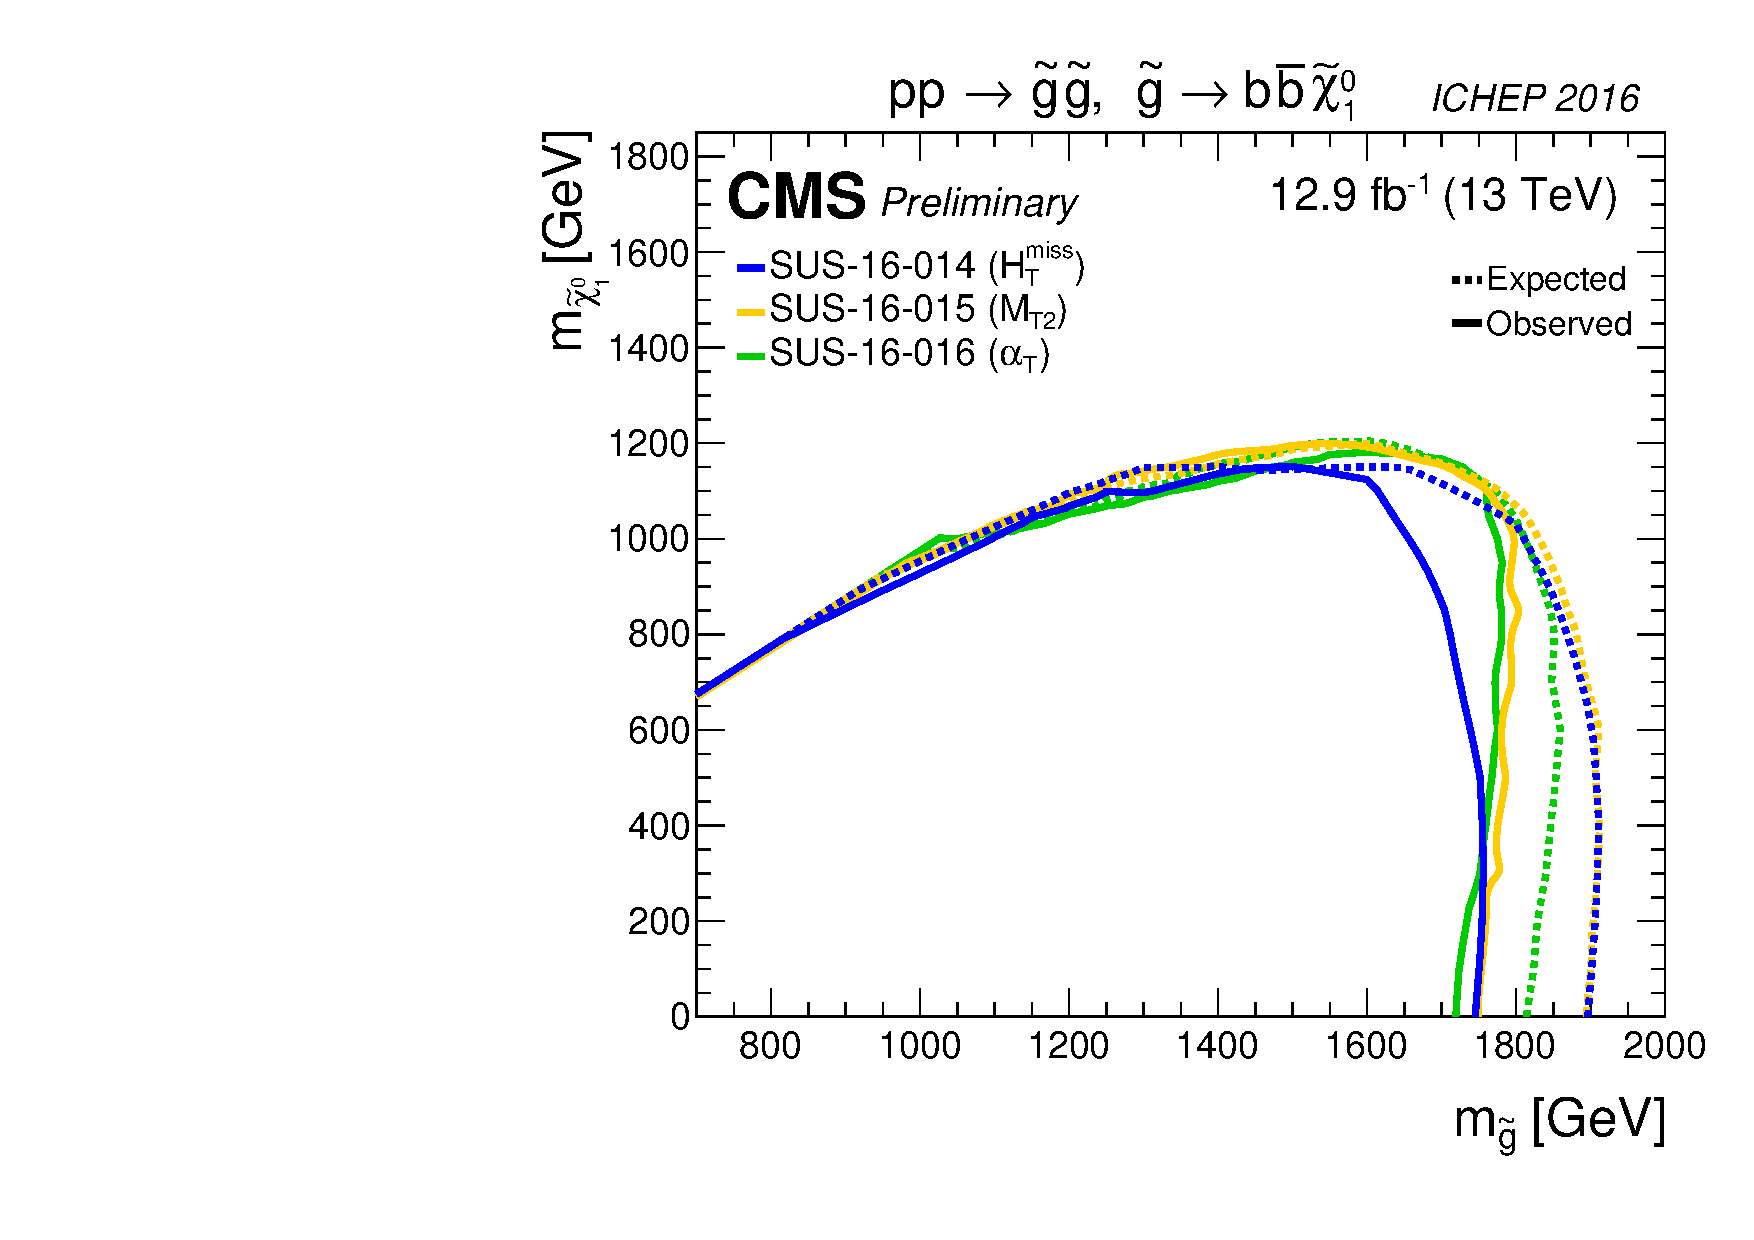
\includegraphics[width=0.45\textwidth]{./Figures/statisticalResults/T1bbbb_limits_summary_cms_ICHEP16} ~
    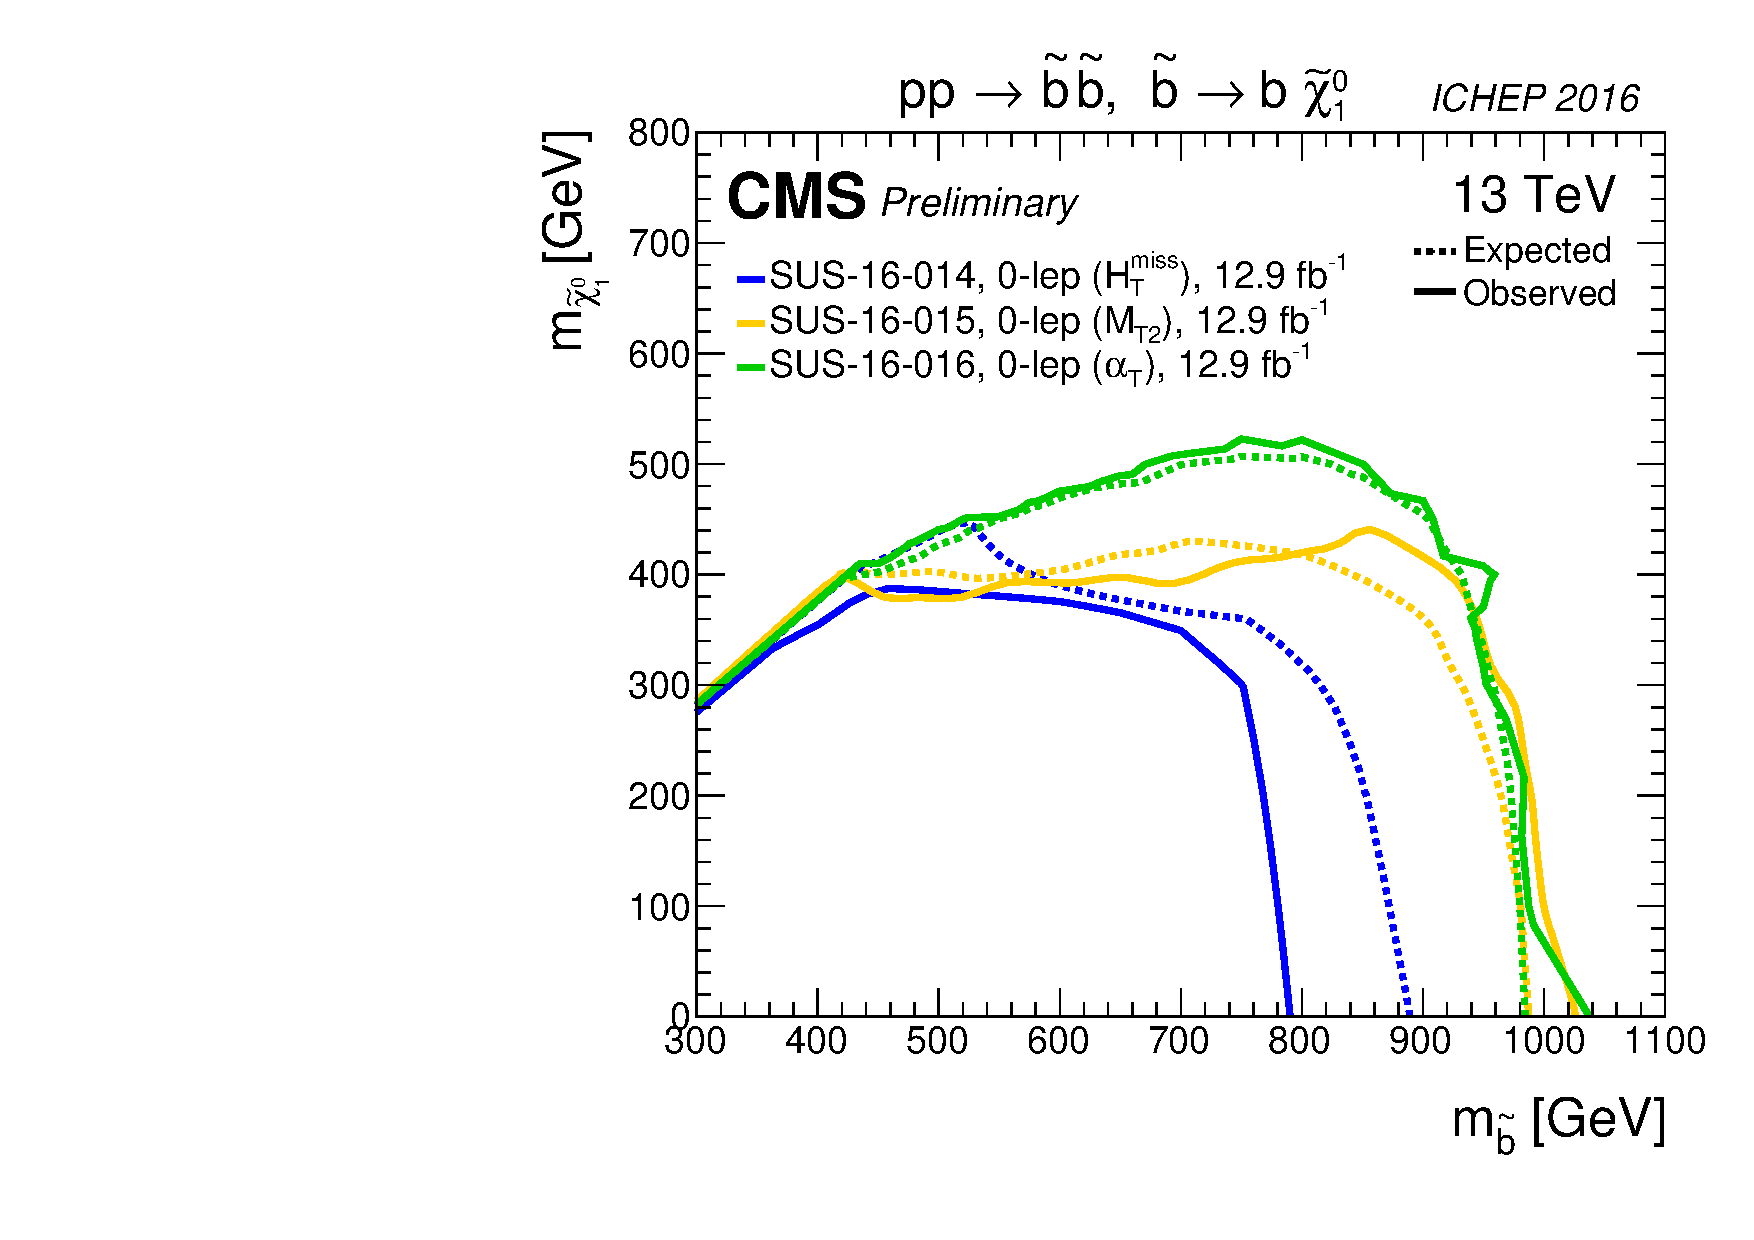
\includegraphics[width=0.45\textwidth]{./Figures/statisticalResults/T2bb_limits_summary_cms_ICHEP16}
    \caption{Observed and expected exclusion contours at 95\% confidence
      level (indicated by the colour scale) for simplified models that
      assume the (Left) gluino-mediated or (Right) direct production
      bottom, as a function of the gluino or squark mass and the $\chiz_{1}$ 
      mass. The results from the \alphat~analysis are compared to 
      the \mtt and \htmiss analyses~\cite{mt2,ra2}. \label{fig:limits-sms-competition} }
  \end{center}
\end{figure}
